\labsection{Диа- и парамагнетизм}

Одной из основных макроскопических характеристик веществ, которая используется для описания их магнитных свойств, является вектор намагниченности $\vec{M}$~--- суммарный магнитный момент единичного объёма вещества. В ряде веществ между намагниченностью $M$ и напряжённостью магнитного поля $H$ имеет место линейная зависимость.
\todo [author=Tiffani]{Здесь не хватает формулы 4.1 ($\vec{M} = \chi\vec{H}$), на которую ссылаются ниже. Формулу добавила из старой версии лабника.}
\begin{equation}
	\eqmark{magnetization-magnetic vector}
	\vec{M} = \chi\vec{H}.
\end{equation}

\begin{wrapfigure}[23]{r}{0.35\textwidth}
	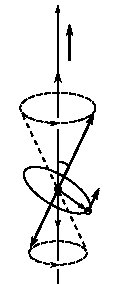
\includegraphics[width=0.2\textwidth]{v4_1}
	\caption{Прецессия электронной орбиты в магнитном поле}
	\figmark{electron orbit}
\end{wrapfigure}

Рассмотрим одну из электронных орбит атома. Пусть электрон с зарядом $-e$ и массой $m_e$ движется со скоростью $v$ по круговой орбите радиуса $r$, а его орбитальный момент количества движения $L$ лежит в плоскости рис.~\figref{electron orbit} и направлен под углом $\theta$ к некоторой оси $z$. С моментом импульса $L$ связан орбитальный магнитный момент, который направлен в противоположную сторону, поскольку заряд электрона отрицательный. При включении магнитного поля с индукцией $B$, направленной вдоль оси $z$, на атом начинает действовать механический момент
\todo [author=Tiffani]{Нет подписи под рисунком 4.1. Добавила из старой версии лабника. Проверить. Обозначения на рис. неправильные.}
\begin{equation*}
	N = \vec{\mu}_L\times \vec{B},
\end{equation*}
который перпендикулярен плоскости рис.~\figref{electron orbit} и направлен от нас. Уравнение движения атома будет иметь вид
\begin{equation*}
	\frac{d\vec{L}}{dt} = \vec{\mu}_L\times \vec{B}.
\end{equation*}

Аналогичное хорошо известное в механике уравнение описывает угловую прецессию волчка. В нашем случае это уравнение описывает прецессию электронной орбиты с угловой частотой
\begin{equation*}
	\Omega_L = \frac{\mu_L B}{L}
\end{equation*}
и направленной вдоль магнитного поля. Поскольку $L = m_e vr$, а  $\mu_L =~1/2evr$, то
\begin{equation*}
	\Omega_L = \frac{Be}{2m_e}.
\end{equation*}
Эта частота называется \important{ларморовой угловой частотой}. Следует отметить, что ни направление, ни величина ларморовой угловой частоты не зависят от угла $\theta$.
Прецессия электронной орбиты приводит к дополнительному вращению электрона вокруг поля $B$, налагающемуся на его орбитальное движение.  Это дополнительное движение эквивалентно замкнутому току. Прецессия электронной орбиты приводит к дополнительному вращению электрона вокруг поля $B$, налагающемуся на его орбитальное движение. Это дополнительное движение эквивалентно замкнутому току $\Delta i$ в плоскости, перпендикулярной вектору $B$:
\begin{equation*}
	\Delta i = - \frac{e\Omega_L}{2\pi} = - \frac{e^2}{4\pi m_e}B.
\end{equation*}
Этот ток создает магнитный момент
\begin{equation*}
	\Delta\mu_L = \Delta i \cdot S = - \frac{e^2 S}{4\pi m_e}B = - \frac{\mu_0 e^2 S}{4\pi m_e}H,
\end{equation*}
где $S$~--- площадь контура, который описывает электрон в результате прецессии вокруг поля $B$. Если рассматривать сферически-симметричное распределение заряда электрона, то расчёт показывает, что $S = 2/3\pi\average{r^2}$, где $\average{r^2}$~--- средний квадрат расстояния электрона от ядра. Поэтому
\begin{equation*}
	\Delta\mu_L = - \frac{\mu_0 e^2 \average{r^2}}{6m_e}H.
\end{equation*}

Появление этого момента и приводит к намагничиванию вещества в направлении, противоположном полю, т.е. к диамагнетизму. Магнитный момент атома, содержащего $Z$ электронов, находится суммированием магнитных моментов отдельных электронов:
\begin{equation*}
	\mu_{\text{ат}} = - \frac{\mu_0 e^2 H}{6m_e}\sum\limits_{i=1}^Z \average{r_i^2}.
\end{equation*}

Сумму можно заменить произведением $Z\average{a^2}$, где $\average{a^2}$~--- средний квадрат расстояния электронов от ядра. Тогда
\begin{equation*}
	\mu_{\text{ат}} = - \frac{\mu_0 e^2 \average{a^2} Z}{6m_e}H.
\end{equation*}
Умножив полученное выражение на число атомов $n$ в единице объёма, получим намагниченность $M$:
\begin{equation*}
	M = n\mu_{\text{ат}} = - \frac{\mu_0 e^2 \average{a^2} nZ}{6m_e}H.
\end{equation*}
Магнитная восприимчивость
\begin{equation*}
	\chi = \frac{M}{H} = - \frac{\mu_0 e^2 \average{a^2} nZ}{6m_e}.
\end{equation*}
Положив $a \sim 10^{-10}$~м, $n \sim 5 \cdot 10^{-28}$~м$^3$, получим, что $\chi \approx -10^{-6}~Z$.

Эта оценка находится в хорошем согласии с экспериментальными результатами.
Из полученного выражения для магнитной восприимчивости диамагнетиков следует, что она не зависит ни от температуры, ни от величины напряжённости поля и растёт пропорционально порядковому номеру элемента.
Диамагнитный эффект свойствен всем веществам (независимо от того, имелся ли у атома собственный магнитный момент или нет и как он был ориентирован), однако у некоторых веществ он перекрывается более сильным \important{парамагнитным} эффектом. В отличие от диамагнетизма парамагнетизм характерен для веществ, частицы которых (атомы, ионы, молекулы) обладают собственным магнитным моментом в отсутствие внешнего магнитного поля. Этот магнитный момент обусловлен как движением электронов в оболочке атома (орбитальный магнитный момент), так и наличием собственных магнитных моментов у электронов и ядер (\important{спиновый} магнитный момент). Например, в кристаллах медного купороса (CuSO$_4$) содержатся ионы меди, у которых электроны на внутренних оболочках имеют суммарный магнитный момент, не равный нулю. Изолированный атом меди имеет нечётное число электронов (29). На внешней оболочке $4s$ имеется всего один электрон, и именно его магнитный момент является магнитным моментом атома меди. Поэтому пары меди, как и пары натрия, являются парамагнетиками. Однако при переходе в твёрдое состояние (в процессе кристаллизации) атомы меди теряют этот электрон, он уходит от своего атома и уже принадлежит всему кристаллу. «Застывшие» в узлах решётки ионы меди уже не имеют магнитного момента и поэтому не обладают парамагнитным эффектом. Обобществлённые электроны (электроны проводимости) образуют электронный газ, который является парамагнетиком, поскольку состоит из частиц, обладающих собственным магнитным моментом. Такой парамагнетизм называют \important{парамагнетизмом Паули}. Но медь является диамагнетиком, и это означает, что диамагнетизм ионов меди преобладает над парамагнетизмом свободных электронов.

Отличительной особенностью парамагнетиков является их слабая намагниченность во внешнем магнитном поле при комнатной температуре. В отсутствие магнитного поля энергия диполь-дипольного взаимодействия между двумя соседними магнитными моментами атомов с межатомным расстоянием $\sim 5 \cdot 10^{-8}$~см составляет $\sim 10^{-5}$~эВ, а энергия
теплового движения на атом $\sim 7,5 \cdot 10^{-2}$~эВ. Такое превосходство тепловой энергии приводит к равномерному пространственному распределению магнитных моментов, а следовательно, к отсутствию намагниченности у парамагнетиков. Но когда начинает действовать внешнее магнитное поле, оно выстраивает магнитные моменты так, что магнитных моментов, направленных по полю, становится больше, чем направленных против поля, и с ростом поля намагниченность парамагнетиков растёт по закону \eqref{magnetization-magnetic vector}.
Магнитная восприимчивость парамагнетиков всегда положительна, а по величине $\chi \sim 10^{-6} \sim 10^{-4}$~(система СИ).

Найдём температурную зависимость магнитной восприимчивости парамагнетика. Пусть среднее число атомов в единице объёма равно $N$, а абсолютная величина магнитного момента атома $\mu_{\text{Б}}$. В магнитном поле с индукцией $B$ энергия магнитного диполя, составляющего с направлением поля угол $\alpha$,

\begin{equation*}
	U = - \mu_{\text{Б}}B \cos \alpha.
\end{equation*}
\todo [author=Tiffani]{Нет рисунка 4.2. Добавила. Проверить. Подписи к рисунку нет. Обозначения на рис. неправильные}
\begin{wrapfigure}[]{r}{0.35\textwidth}
	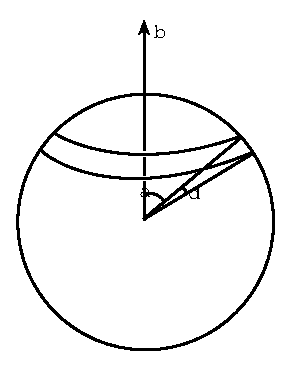
\includegraphics[width=0.2\textwidth]{v4_2}
	\caption{Подписи к рисунку нет}
	\figmark{dN in dOmega}
\end{wrapfigure}

Используя распределение Больцмана, запишем число атомов из единичного объёма, магнитные моменты которых направлены под углами от $\alpha$ до $\alpha + d\alpha$ в малом телесном угле $d\Omega = 2\pi\sin \alpha~d\alpha$ (рис.~\figref{dN in dOmega}):
\begin{equation*}
	dN = N_0 \exp \left( \frac{\mu_{\text{Б}}\cos \alpha}{kT}\right)2\pi \sin \alpha~d\alpha,
\end{equation*}
где $N_0$ -- нормировочная константа.

Полное число атомов в единице объёма
\begin{equation}
	\eqmark{total number of atoms}
	N = 2\pi N_0 \int\limits_0^\pi e^{\frac{\mu_{\text{Б}} B \cos \alpha}{kT}} \sin \alpha~d\alpha.
\end{equation}

Поскольку проекция магнитного момента атома на направление поля равна $\mu_{\text{Б}} \cos \alpha $, то суммарный магнитный момент всех атомов единицы объема будет равен
\begin{equation}
	\eqmark{total magnetic moment}
	M = 2\pi N_0 \int\limits_0^\pi \mu_{\text{Б}} \cos \alpha \exp \left(\frac{\mu_{\text{Б}} B \cos \alpha}{kT}\right) \sin \alpha~d\alpha.
\end{equation}

Магнитный момент электрона $\mu_{\text{Б}} = e\hbar/2m_e = 9,27 \cdot 10^{-24}$ А $\cdot$~м$^2$ (магнетон Бора). В магнитном поле с индукцией $B = 1,0$~Тл магнитная энергия $\mu_{\text{Б}}~B \sim \mathbf{10^{-4}}$~эВ. Поэтому в не слишком больших полях и не слишком низких температурах показатель экспоненты много меньше единицы. 

В этом приближении из совместного решения \eqref{total number of atoms} и \eqref{total magnetic moment} получим, что намагниченность
\begin{equation*}
	M \approx \frac{\mu_{\text{Б}}^2 \mu_0 BN}{3kT} = \frac{\mu_{\text{Б}}^2 \mu_0 N}{3kT} H.
\end{equation*}
Магнитная восприимчивость
\begin{equation*}
	\chi = \frac{M}{H} = \frac{\mu_{\text{Б}}^2 \mu_0 N}{3kT}.
\end{equation*}
Температурная зависимость восприимчивости парамагнетиков вида $1/T$ называется законом Кюри.

В очень сильных полях, когда магнитная энергия внутриатомного диполя сравнима с тепловой ($B \sim 10^3$~Тл при комнатной температуре), все магнитные моменты в парамагнетике могут ориентироваться по полю~--- наступает магнитное насыщение.

В случае парамагнетизма свободных электронов, образующих электронный газ в металлах, не все электроны могут участвовать в переориентировке своих магнитных моментов, а только небольшая часть, которая пропорциональна тепловой энергии $kT$ (квантовый эффект). Поэтому у некоторых металлов парамагнетизм не зависит от температуры.

\labsection{Ферромагнетизм}

Помимо диа- и парамагнетиков, которые слабо реагируют на внешнее магнитное поле, в природе существуют вещества, способные сильно намагничиваться даже в небольших магнитных полях. Такие вещества относят к классу ферромагнетиков. Это~--- железо, никель, кобальт, гадолиний и многочисленные сплавы этих металлов между собой и с другими металлами. Ферромагнитными свойствами обладают некоторые сплавы элементов, которые порознь не являются ферромагнитными (например, сплавы меди и марганца), и ряд неметаллических веществ (ферриты).

Зависимость намагниченности $M$ от напряжённости магнитного поля $H$ у всех ферромагнетиков оказывается нелинейной, поскольку магнитная восприимчивость $\chi$ у ферромагнетиков не является константой и зависит от $H$. Если у диа- и парамагнетиков $\chi$ составляет всего $10^{-8}$~--~$10^{-3}$, то у ферромагнетиков магнитная восприимчивость достигает значений $10^4$~--~$10^5$. Кроме того, у ферромагнетиков (особенно монокристаллических) наиболее ярко проявляется тензорный характер магнитной восприимчивости $\chi$, обусловленный анизотропией вещества. Степень намагничивания ферромагнитного вещества можно характеризовать не только вектором намагниченности $M$, но и вектором магнитной индукции $B$ в данном веществе:
\begin{equation*}
	B =\mu_0 (H + M).
\end{equation*}
При $M = \chi H$
\begin{equation}
	B = \mu_0 (1 + \chi)H = \mu \mu_0 H.
\end{equation}
\todo [author=Tiffani]{В формуле 4.4 была ошибка. Исправила.}

Величина $\mu = 1+ \chi$ носит название магнитной проницаемости вещества. Если у диа- и парамагнетиков $\mu$ отличается от единицы всего на сотые доли процента, то у ферромагнетиков $\mu$ практически совпадает с $\chi$ (в системе СИ).

Отметим, что в системе СГС, где $B = (1 + 4\pi \chi) H$, $\chi$ в $4\pi$ раз меньше, чем в системе СИ.

Атомы ферромагнетика, как и атомы парамагнетика, обладают собственным магнитным моментом и в отсутствие внешнего магнитного поля. Учёт взаимодействия  элементарных магнитных моментов, заключающийся в прибавлении к макроскопическому полю $H$ поля, пропорционального намагниченности (подобно приёму учёта поля соседей в диэлектрике введением поля поляризуемости с коэффициентом $4\pi/3$), противоречит опыту, поэтому вводится эмпирическая постоянная $\lambda$, т.е. вместо поля $H$ нужно использовать величину $H + \lambda M$.  Используя полученную формулу для намагниченности, получим
\begin{equation*}
	M = \frac{\mu_{\text{Б}}^2 \mu_0 N}{3kT}(H + \lambda M)
\end{equation*}
и соответственно
\begin{equation*}
	\chi = \frac{\mu_{\text{Б}}^2 \mu_0 N}{3k(T - \Theta)},
\end{equation*}
где $\Theta = \mu_{\text{Б}}^2 \mu_0 N / 3k$ имеет размерность температуры.

Зависимость  $1/\chi$  от температуры называется законом Кюри-Вейса и представляется прямой, пересечение которой с осью абсцисс определяет характеристическую температуру. Если эта величина положительна, существует температура, ниже которой восприимчивость принимает огромные значения. Это справедливо для ферромагнетиков, остальные вещества ведут себя подобным образом  вблизи абсолютного нуля. Для $T>\Theta$ ферромагнетики ведут себя как парамагнетики.

Результаты экспериментов для постоянной $\lambda$ для ферромагнетиков дают величину $10^4$, т.е.поле, пропорциональное намагниченности, оказывается порядка $10^7$~эрстед (хотя поле соседних узлов решетки около $10^3$~эрстед).

Огромная величина поля, связанная с намагниченностью, нашла своё объяснение в квантовой теории при введении так называемого обменного взаимодействия электронов, т.е. эти силы имеют электростатическую природу. Характерная энергия этого взаимодействия порядка $10^{-13}$~эрг. В результате этого взаимодействия устойчивое состояние ферромагнетика соответствует полной намагниченности, хотя в реальности   оказываются намагничены микроскопические области размером порядка несколько микрометров, а в целом образец ненамагничен. Следует  отметить, что величина магнитного поля в домене примерно совпадает с полем насыщения ферромагнетика. Области полной намагниченности назвали доменами, размер которых является следствием конкурирующих вкладов в полную энергию ферромагнетика: обменной энергии, энергии анизотропии и магнитной энергии. Пример разбиения кристалла на домены приведён на рисунке (??4.3.1??), где полная энергия уменьшается от a) до в). 
\todo [author=Tiffani]{Присутствует ссылка на рис. 4.3.1, которого нет в папке. См. примечание ниже.}

\todo [author=Tiffani]{Здесь должна быть картинка 4.3.1, но она не соответствует той, что в ворде. Нужную картинку в папке с картинками не нашла.}

\begin{wrapfigure}[]{r}{0.5\textwidth}
	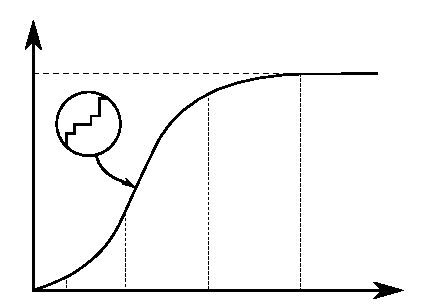
\includegraphics[width=0.4\textwidth]{v4_3}
	\caption{Начальная кривая намагничивания ферромагнетика}
	\figmark{magnetization curve}
\end{wrapfigure}

Помимо обменных (близкодействующих) сил между атомами действуют дальнодействующие силы магнитного диполь-дипольного взаимодействия. Энергия такого взаимодействия будет минимальной при антипараллельном расположении магнитных моментов соседних атомов. Поэтому при определённом поперечном (перпендикулярном магнитному моменту) размере домена оказывается энергетически выгодно иметь соседний домен с противоположно направленным магнитным моментом.

Между доменами существуют переходные слои (в железе их толщина $\sim 10^{-5}$~см), в которых направление магнитного момента атомов плавно переходит от направления в одном домене к направлению в соседнем. Такие слои называют «стенками Блоха». Энергия этих слоёв пропорциональна их площади.

\todo [author=Tiffani]{Неплохо было бы выделять термины вроде «стенками Блоха» и «скачки Баркгаузена» курсивом или жирным шрифтом при первом упоминании в тексте.}

Суммарный магнитный момент ферромагнитного образца в отсутствие внешнего магнитного поля неоднозначен: его величина и направление зависят от предыстории образца. В одних случаях он равен нулю (полностью размагниченный образец), а в другом случае он может иметь очень большое значение (например, постоянный магнит).

Если ферромагнетик, находящийся в состоянии полного размагничивания ($M = 0$), намагничивать в медленно нарастающем магнитном поле, то мы получим зависимость $M(H)$, которую называют начальной кривой намагничивания. Эту кривую обычно разделяют на пять условных участков (рис.~\figref{magnetization curve}). Участок I~--- область обратимого намагничивания, где $M =\chi \sim H$. В этой области происходят процессы упругого смещения границ доменов: увеличивается размер тех доменов, магнитный момент которых близок к направлению магнитного поля, и уменьшаются размеры доменов с противоположным направлением магнитного момента. Участок II характеризуется квадратичной зависимостью $M$ от $H$. В этой области также идёт процесс смещения границ, но одновременно как обратимый, так и необратимый. Область максимальной скорости роста намагниченности (III) соответствует необратимым смещениям «стенок Блоха»: им приходится преодолевать «препятствия» в виде примесей, дислокаций и дефектов кристаллической решётки. Когда стенка наталкивается на такое препятствие, она останавливается и держится, пока поле не достигнет определённого значения, при котором она внезапно срывается. Таким образом, движение доменной стенки приобретает скачкообразный характер (скачки Баркгаузена).

Фрагмент кривой намагничивания в этой области в увеличенном масштабе показан на рис.~\figref{magnetization curve}. Скачкообразное движение стенок приводит к быстрому изменению намагниченности образца, что вызывает появление вихревых токов, а следовательно, диссипацию энергии. Выделение тепла внутри образца и приводит к необратимому движению доменных стенок.

 В достаточно сильных полях движение стенок прекращается и энергетически выгодным становится поворот магнитных моментов тех оставшихся доменов, у которых магнитный момент не совпадает с направлением поля (область IV). И, наконец, при некотором значении поля (участок V) все магнитные моменты выстраиваются по полю~--- намагниченность образца достигает насыщения.

\begin{wrapfigure}[12]{r}{0.35\textwidth}
	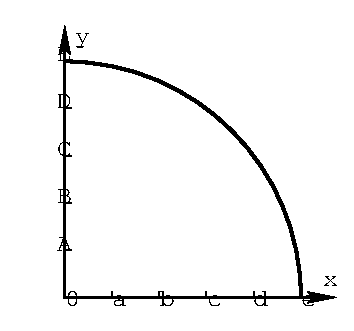
\includegraphics[width=0.2\textwidth]{v4_4}
	\caption{Зависимость намагниченности насыщения ферромагнетика от температуры}
	\figmark{magnetization-temperature}
\end{wrapfigure}

Магнитные и другие физические свойства ферромагнетиков существенным образом зависят от температуры. Например, намагниченность насыщения $M_s$ имеет наибольшее значение при $T = 0~(M_s (0))$ и монотонно уменьшается до нуля при температуре $\Theta$, которую называют ферромагнитной точкой Кюри (рис.~\figref{magnetization-temperature}). 

\todo [author=Tiffani]{Обозначения на рис. 4.4 не имеют ничего общего с действительностью.}

Выше  этой температуры $\Theta$ тепловое движение разупорядочивает магнитную структуру доменов и ферромагнетик переходит в парамагнитное состояние. В отсутствие внешнего магнитного поля переход ферромагнетик~---парамагнетик является фазовым переходом II рода.

Мы уже знаем, что для парамагнетиков зависимость магнитной восприимчивости от температуры имеет вид закона Кюри ($\chi \sim 1/T$). Аналогичная зависимость восприимчивости ферромагнетиков от температуры при температурах выше $\Theta$ описывается законом Кюри-Вейсса:
\begin{equation*}
	\chi = \frac{C}{T - \Theta_p},
\end{equation*}
где $C$ -- постоянная Кюри, $\Theta_p$ -- температура Кюри (как правило $\Theta_p > 0$).

На практике магнитные свойства ферромагнетиков обычно изучают путём измерения зависимости индукции магнитного поля $B$ от напряжённости магнитного поля $H$ в веществе ($B = f(H)$). Исследование образца, естественно, начинают с полностью размагниченного состояния ($H = 0$, $B = 0$). Если теперь монотонно увеличивать напряжённость поля $H$, то изменение $B$ происходит по известной нам начальной кривой намагничивания (кривая $OA$ на рис.~\figref{hysteresis curve}).

\todo [author=Tiffani]{В подписи к рис. 4.5 наверное ``кривая намагниченности'', а не ``кривая намагничения''. Исправила. Проверить.}

\begin{wrapfigure}{r}{0.4\textwidth}
	\pic{0.38\textwidth}{v4_8}
	\caption{Начальная кривая намагниченности и кривая гистерезиса}
	\figmark{hysteresis curve}
\end{wrapfigure}

Эта кривая практически совпадает с кривой намагничивания на рис.~\figref{magnetization curve}, поскольку вклад $B$ в намагниченности $M$ существенно больше, чем $H$. Скорость подъёма кривой $OA$ характеризуется  дифференциальной магнитной проницаемостью
\begin{equation*}
	\mu_{\text{дифф}} = \frac{1}{\mu_0} \frac{dB}{dH}.
\end{equation*}

Дифференциальная магнитная проницаемость обычного железа с ростом $H$ сначала увеличивается, а затем начинает резко падать, приближаясь к единице при насыщении. Дойдя до некоторой точки $A$, лежащей достаточно далеко в области насыщения (здесь $B_s$~--- индукция насыщения)\footnote[1]{s~--- saturated (англ.)~--- насыщенный}, начнём уменьшать напряжённость поля $H$.
 Обратный путь не идёт по начальной кривой, а проходит выше неё.
 
 \todo [author=Tiffani]{Термины ``индукция насыщения'', ``остаточной индукции'' и ``коэрцетивной силы'' лучше выделить курсивом или жирным шрифтом.}
 \todo [author=Tiffani]{Сноски оформила через footnote. Текста сносок в ворде не было, взяла из старой версии лабника. Однако, сноски не несут особой инофрмации, может их лучше убрать?}
 
При $H = 0$ в образце сохраняется некоторое намагничивание. Величина $B_r$, достигаемая в точке $H = 0$ при возвращении из состояния насыщения, носит название остаточной индукции\footnote[2]{r~--- remained (англ.)~--- оставшийся}. Значение $B = 0$ достигается лишь при некотором отрицательном значении $H = - H_c$. Величина $H_c$ называется коэрцитивной силой\footnote[3]{c~--- coercive (англ.)~--- принудительный}. Среди ферромагнетиков принято различать магнитожёсткие (с $H_c > 10^3$~А/м) и магнитомягкие матералы. В точке $C$ наступает насыщение для намагничивания в противоположную сторону.

Постараемся теперь вернуться в точку $A$. Магнитное состояние вещества характеризуется теперь точками кривой $CA$, лежащими низке начальной кривой намагничивания. Строго говоря, кривая не пройдёт и через точку $A$, а окажется ниже неё. Вновь уменьшая магнитное поле, мы пройдём поэтому по кривой, расположенной ниже кривой $AC$, не попадём в точку $C$ и начнём движение к $A$ по некоторому новому пути. Магнитные циклы, таким образом, обычно оказываются незамкнутыми. Многократно проходя один и тот же цикл, образец приближается к предельному замкнутому циклу (кривой гистерезиса), не зависящему от начального состояния. Описанная картина наиболее отчётливо проявляется в тех случаях, когда образец не доводится до насыщения. При заходе в область насыщения намагничивание зависит главным образом от $H$ и лишь в очень слабой степени от истории образца. Предельные циклы устанавливаются при этом сразу (т. е. при однократном прохождении цикла) или почти сразу. В соответствии с этим на рис.~\figref{magnetization curve} не сделано различия между частным циклом и предельным.

Можно показать, что площадь петли гистерезиса пропорциональна энергии, теряемой в единице объёма вещества за время цикла:
\begin{equation*}
	\text{??Здесь должна быть какая-то формула??}.
\end{equation*}
Действительно, если к соленоиду с длиной $l$ подсоединён источник напряжения с эдс $\mathscr{E}$, сечением $S$ и числом витков N, отбираемую от источника мощность можно записать так

 \todo [author=Tiffani]{ Есть путаница с тремя последними формулами в этом разделе. Надо разобраться.}
\begin{equation*}
	\frac{dW}{dt} = \mathscr{E} \cdot I = NS \frac{dB}{dt} \cdot I = lSH \frac{dB}{dt}.
\end{equation*}
Тогда в единице объёма энергия потерь за цикл
\begin{equation*}
	w = \oint {HdB}.
\end{equation*}

\labsection{Размагничивающий фактор}

Когда мы говорим о кривой намагничивания $B(H)$ какого-то ферромагнитного материала, то речь идёт о локальной связи между индукцией и величиной магнитного поля внутри этого вещества. Подчеркнём, что в зависимости $B(H)$ имеется в виду не внешнее магнитное поле, а именно поле внутри данного материала. На практике для снятия петли гистерезиса мы обычно помещаем во внешнее однородное магнитное поле ферромагнитный образец, имеющий конечные размеры. Однородная намагниченность по всему объёму образца будет иметь место только для образцов, имеющих форму эллипсоидов вращения, в частности, для шара, для очень тонкой пластинки и для тонкого и длинного цилиндра. Во всех этих случаях величина магнитного поля внутри образца будет меньше внешнего магнитного поля. Рассмотрим в качестве примера образец, имеющий форму цилиндра длиной $l$ и диаметром $d (d \ll l)$.

Пусть ось симметрии цилиндра направлена вдоль внешнего магнитного поля величиной $H_0$. Цилиндр будет практически однородно намагничен с некоторой намагниченностью $M$. Найдём величину индукции магнитного поля на оси цилиндра в точке, равноудалённой от торцов. С одной стороны, используя связь между $B$, $M$ и $H$, можно записать
\begin{equation}
	\eqmark{cylinder-B(H)}
	B_{\text{вн}} = \mu_0 (H_{\text{вн}} + M),
\end{equation}
где $H_{\text{вн}}$~--- величина поля внутри образца. С другой стороны, намагниченный цилиндр можно рассматривать как цилиндрическую поверхность диаметра $d$ с однородным кольцевым поверхностным током плотностью:
\begin{equation*}
	j = M.
\end{equation*}
Эти молекулярные токи создают собственное магнитное поле, которое по направлению совпадает с внешним полем $H_0$, а по величине равно\footnote[4]{См. [4]. Задача № 5.5.}:

\todo [author=Tiffani]{Возможно, лучше вместо ``См. [4]. Задача № 5.5.'' написать ``См. в приложении'', т.к. задача будет в приложении к этой главе}
\begin{equation*}
	H_{\text{мол}} = \frac{Ml}{\sqrt{l^2 + d^2}}.
\end{equation*}

Индукцию магнитного поля найдём как суперпозицию внешнего поля и поля молекулярных токов:
\begin{equation}
	\eqmark{B(H)-molecular current}
	B_{\text{вн}} = \mu_0\left( H_0 + \frac{Ml}{\sqrt{l^2 + d^2}} \right).
\end{equation}
Приравнивая \eqref{cylinder-B(H)} и \eqref{B(H)-molecular current}, получим
\begin{equation*}
	H_0 + \frac{Ml}{\sqrt{l^2 + d^2}} = H_{\text{вн}} + M.
\end{equation*}

Разность между внешним и внутренним полями называют размагничивающим полем:
\begin{equation*}
	H_{\text{разм}} = H_0 - H_{\text{вн}} = \left( 1 - \frac{1}{\sqrt{1 + \left( \frac{d}{l} \right)^2}} \right) M = N_p M.
\end{equation*}
И тогда связь поля внутри и поля внешнего
\begin{equation*}
	H_{\text{вн}} = \frac{H_0}{1 + N_p M},
\end{equation*}
а  магнитная проницаемость образца
\begin{equation*}
	\chi_{\text{обр}} = \frac{\chi}{1 + N_p \chi}.
\end{equation*}
\important{Коэффициент пропорциональности между размагничивающим полем и намагниченностью образца обозначают через $N_p$ и называют размагничивающим фактором или коэффициентом размагничивания. Его величина зависит только от геометрических размеров образца и может изменяться в пределах от 0 до 1.}

Полученное выражение для $N_p$ цилиндра с параметрами $d/l \ll 1$ всё равно остаётся приближённым выражением, хотя и с достаточно хорошим приближением. А вот точные значения размагничивающего фактора могут быть рассчитаны только в отдельных частных случаях:

\begin{wrapfigure}[13]{r}{0.4\textwidth}
	\pic{0.38\textwidth}{v4_5}
	\caption{Тороидальный образец с намагничивающей обмоткой}
	\figmark{toroid}
\end{wrapfigure}

\begin{enumerate}
	\item бесконечно длинный цилиндр с конечным размером диаметра: 
в случае продольного внешнего магнитного поля $N_p = 0$, в случае 
поперечного~--- $N_p = 1/2$;

	\item для шара $ N_p = 1/3$;
	
	\item в случае бесконечно тонкой пластинки при поперечном внешнем магнитном поле $N_p = 1$, а при продольном --- $N_p = 0$.
\end{enumerate}

В лабораторных условиях для исследования зависимости $B(H)$ ферромагнитных материалов обычно используют образцы тороидальной формы. Если на тор намотать равномерную намагничивающую обмотку (рис.~\figref{toroid}), то поле $H$ внутри тора на окружности радиуса $R$ будет пропорционально току $I$ в обмотке, а его величину можно рассчитать по теореме о циркуляции вектора $H$:
\begin{equation}
	\eqmark{H-toroid}
	H = \frac{IN_0}{2\pi R},
\end{equation}
где $N_0$~--- число витков намагничивающей обмотки. Напряжённость магнитного поля в тороидальном образце зависит от $R$, поэтому при $r \ll R$ мы будем иметь достаточно однородную намагниченность образца.

\labsection{Измерение напряжённости магнитного поля в образцах}

Пусть ширина разреза $S$ существенно меньше радиуса сечения тора $r$, который в свою очередь мал по сравнению со средним радиусом тора $R$. Обозначим ферромагнитный образец, имеющий форму тора с поперечным разрезом (рис.~\figref{toroidal coil-cut}).

\begin{wrapfigure}{r}{0.4\textwidth}
	\pic{0.38\textwidth}{v4_6}
	\caption{Тороидальная катушка с разрезом}
	\figmark{toroidal coil-cut}
\end{wrapfigure}

Обозначим через через $N_0$ число витков намагничивающей обмотки и через $I$~--- силу намагничивающего тока. Пусть $H$~--- напряжённость магнитного поля в образце, а $H_2$~--- в зазоре. По теореме о циркуляции вектора $H$ имеем
\todo [author=Tiffani]{В уравнении 4.8 необходим знак интеграла по контуру. Исправила. Проверить.}
\begin{equation}
	\eqmark{H-toroid-cut}
	\oint {Hdl} = H_1 (2\pi R - \delta) + H_2 \delta  = N_0 I.
\end{equation}

Чтобы найти из этой формулы $H_1$ и $H_2$, нужно установить связь между ними. Для этого используем нeпрерывность нормальных составляющих вектора магнитной индукции $B$ на границах разреза. Замечая, что в образце $B_1 = \mu_0 \mu H_1$, а в зазоре $B_2 = \mu_0 H_2$, и приравнивая $B_1$ и $B_2$, найдём, что $\mu H_1 = H_2$. Заменяя с помощью этой формулы $H_2$ в формуле \eqref{H-toroid-cut}, получим
\todo [author=Tiffani]{Была пропущена нумерация уравнения 4.9. Исправила.}
\begin{equation}
	\eqmark{H1-toroid-inside}
	H_1 = \frac{N_0 I}{2\pi R + (\mu - 1)\delta},
\end{equation}
и, следовательно,
\begin{equation}
	\eqmark{H2-toroid-gap}
	H_2 = \frac{N_0 I \mu}{2\pi R + (\mu - 1)\delta}.
\end{equation}

Из этих формул следует ряд важных выводов. Отметим, прежде всего, что напряжённости поля в образце и в зазоре (при $\mu = const$) пропорциональны силе намагничивающего тока. После того, как установлена величина коэффициента пропорциональности, измерение напряжённости может быть заменено измерением тока.

В образце без зазора, когда $\delta = 0$,
\todo [author=Tiffani]{Уравнения 4.7 и 4.11 одинаковые.}
\begin{equation}
	\eqmark{H-toroid-without gap}
	H = \frac{IN_0}{2\pi R},
\end{equation}

При наличии даже небольшого зазора второе слагаемое в знаменателе \eqref{H1-toroid-inside} существенно превосходит первое из-за большой величины $\mu$. В этом случае также нетрудно определить напряжённость поля в воздушном зазоре. В самом деле, пренебрегая первым слагаемым в знаменателе \eqref{H2-toroid-gap} по сравнению со вторым и заменяя единицей коэффициент $(\mu - 1)/\mu$, найдём, что в достаточно больших зазорах (т.е. почти всегда)
\begin{equation}
	\eqmark{H2-toroid-big gap}
	H_2 = \frac{N_0 I}{\delta},
\end{equation}

Как следует из формулы \eqref{H2-toroid-big gap}, размеры магнитного ярма (части магнитной цепи, заполненной веществом с большим $\mu$) практически не сказываются на напряжённости магнитного поля в зазоре. Мало сказывается на ней и форма ярма. Поэтому ярма электромагнитов~--- устройств, предназначенных для создания больших магнитных полей в воздушных зазорах,~--- могут иметь самые разные формы.

Воздушные зазоры электромагнитов можно использовать для исследования ферромагнитных образцов.

\labsection{Измерение индукции в образце}

Одним из самых удобных и надёжных методов измерения индукции $B$ является метод, основанный на законе электромагнитной индукции. Электродвижущая сила, возникающая в контуре при изменении пронизывающего контур магнитного потока $\Phi (B)$, равна
\begin{equation}
	\eqmark{EMF-magnetic flux}
	\mathscr{E} = - \frac{d\Phi (B)}{dt},
\end{equation}

Так как магнитный поток $\Phi (B)$ равен произведению индукции $B$ на площадь образца, формула \eqref{EMF-magnetic flux} позволяет определить производную от индукции $B$. Чтобы измерить саму величину $B$, необходимо иметь в составе аппаратуры интегрирующий прибор. В качестве последнего чаще всего применяют милливеберметр (работа 3.4.1) или баллистический гальванометр, отклонение стрелки которого при определённых условиях пропорционально интегралу от протекшего через него тока (работа 3.4.4), или интегрирующую $RC$-цепочку (работа 3.4.5).При этом стоит обратить внимание на то, что для чистых металлов типа железа, имеющих хорошую проводимость и большую магнитную проницаемость, глубина проникновения магнитного поля на частоте 50~Гц около 1~мм. 
\todo [author=Tiffani]{Существуют ли автоматические ссылки на лабораторные работы?} 
\todo [author=Nozik, color=green]{Добавлены автоматические ссылки вида lab:\\thechapter.\\thelab} 